\chapter{Wi-Fi Direct Middleware}
\label{chap2}
\thispagestyle{empty}

\noindent In this section I'll show the low-level architecture of the sPFWFDMid module. With this chapter you'll able to update the middleware in the future. Because, I have completely changed most of the code in this module, you should consider completely deprecated the version of SPF1 and the related documentation.

\section{A quick overview}

All Wi-Fi Direct Middleware is into the sPFWFDMid sub-module. There are two main packages:

\begin{itemize}
	\item wfd: contains the entire logic 
	\item wfdadapter: contains all the classes and interfaces directly related to SPF
\end{itemize}

When you open SPF on your smartphone, the first thing that happens, also before the start of the MainActivity, is the execution of the code into the SPFApp.java, that extends Application. 
The first thing that SPFApp does is inside his Application's class, where there is the initialization of SPF, with this line \textsf{SPFContext.initialize(this, 0, true, WFDMiddlewareAdapter.FACTORY);}. As you can see, the only things that you must provide to this method are:
\begin{itemize}
	\item context: necessary to use all methods that require context into the middleware, where there aren't any ways to get it;
	\item goIntent and isAutonomous: are specificities of Wi-Fi Direct Middleware. I'll talk on that during this document. Obviously, it should be removed in the future;
	\item middleware: to specify the middleware that you want to use. In SPF2, the only available middleware is Wi-Fi Direct.
\end{itemize}


\begin{figure}[thpb]
	\centering
	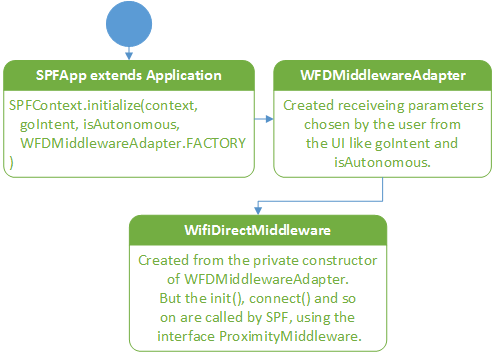
\includegraphics[scale=0.5]{./images/chap2/uml-parte0-1.png}
	\caption{Uml part 0.}
	\label{uml-part0-1}
\end{figure}	

After that, as you can see in Figure \ref{uml-part0-1}, WFDMiddlewareAdapter (the most important class included into the wpdadapter's package of the middleware) will be created and automatically it will instantiate the WifiDirectMiddlware object (the most important class included into the wfd's package of the middleware). This process completes only with the creation of this last object, because the real initialization process and  connection are made by SPF using the ProximityMiddleware interface. 
I'll discuss more in details these aspects in the next session.
At the moment, i want explain only the events used to send messages into the middleware. The main idea was to prevent most of the circular dependencies that Wi-Fi Direct APIs force to use.
To do that i'm using a library called Otto. 
Otto is an event bus designed to decouple different parts of your application while still allowing them to communicate efficiently. Forked from Guava, Otto adds unique functionality to an already refined event bus as well as specializing it to the Android platform.
To be able to post events in all Threads i'm using a wrapper called Ninbus.
But, the only difficulties to use this library is how maintain an ordered structure. 

\begin{figure}[thpb]
	\centering
	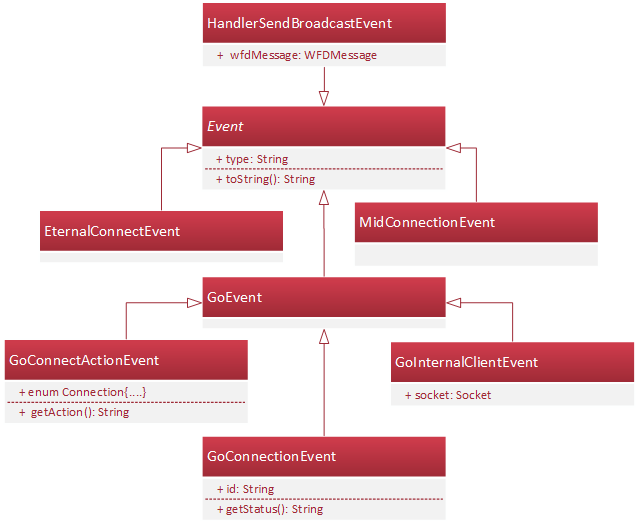
\includegraphics[scale=0.7]{./images/chap2/event-hyerarchy.png}
	\caption{Uml part 0.}
	\label{event-hyeranchy}
\end{figure}	

\begin{figure}[thpb]
	\centering
	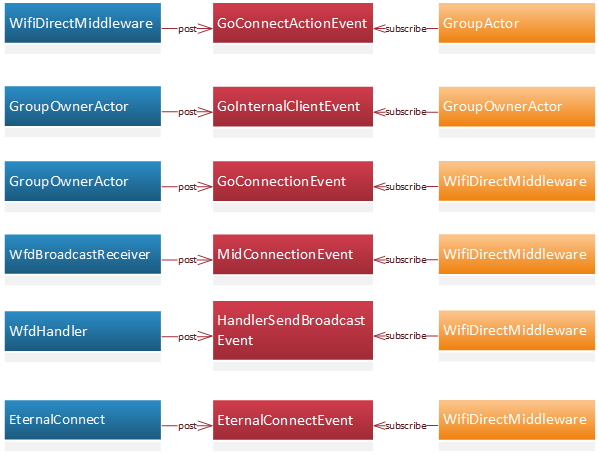
\includegraphics[scale=0.7]{./images/chap2/event-subscribe-post.png}
	\caption{Uml part 0.}
	\label{event-subscribe-post}
\end{figure}	

To achieve this, I use a package with all events inside, organized using the java hierarchy. The complete class diagram all all events is in Figure \ref{event-hyeranchy}.
Another important thing is to undestand which class posts an event and which will react to this event.
To examplain in a very simple way this fact, i created the diagram in Figure \ref{event-subscribe-post}. As you can see:

\begin{itemize}
	\item the blue elements are the classes the post events
	\item in red there are all events
	\item in orange are represented all subscribers
\end{itemize}

This means that, WifiDirectMiddleware.java posts a GoConnectActionEvent and GroupActor will catch the events and it will react to this executing a method annotated with @Subscribe.

\section{Architecture}

\begin{figure}[thpb]
	\centering
	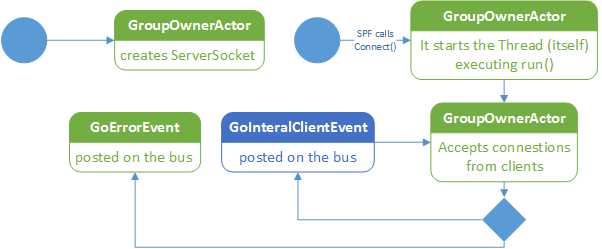
\includegraphics[scale=0.5]{./images/chap2/uml-parte0-2.png}
	\caption{Uml part 0.}
	\label{uml-part0-2}
\end{figure}	

\begin{figure}[thpb]
	\centering
	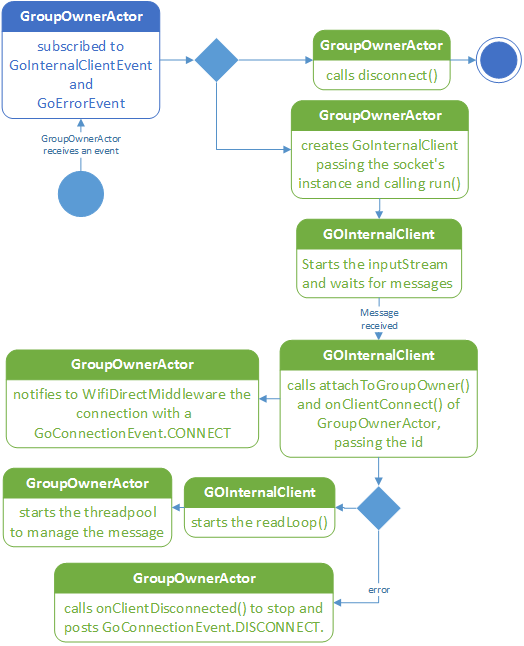
\includegraphics[scale=0.6]{./images/chap2/uml-parte0-3.png}
	\caption{Uml part 0.}
	\label{uml-part0-3}
\end{figure}	

I don't want to explain in details the code of this middleware, instead, I want to examplain the structure and the interactions of the classes inside the wfd/groups package.
I created two different scheme to describe this. They are represented as state diagram because very simple to read, but probably the best type of uml could be the Sequence Digram.
First, I want to describe how GroupActor and its subclasses post events. As you can see in Figure \ref{uml-part0-2}, when GroupOwnerActor start, it will create a ServerSockets, nothing more.
It will be SPF that with the connect method will starts the GroupOwnerActor's thread executing the run() method. Inside of them, it will start to listen and accapt clients connections. If everything will be ok, it will post a GoInternalClientEvent on the bus, instead a GoErrorEvent. In the first case, it will return to listen and accepts other clients, that to the while's cycle. Obviously this is only an extreme abstraction. To understand more in detail this, look the Figure \ref{uml-part0-3} where I represented the sequence of operations that starts when GroupOwnerActor receives the GoInternalClientEvent postes by itself (from is run() method and for this reason from another thread).
When GroupOwnerActor receives this event it will create and starts a GoInternalClient, passing the socket instance.
After that, this last thread starts the InputStream and waits for messages. 
When it receive a message, it calls attachToGroupOwner() and onClientConnect() of GroupOwnerActor, passing the identifier of the profile. These calls are necessary to notify to the WifiDirectMiddlware what happened, but the real logic will continue into the method readLoop() inside the GoInternalClient that start the threadpool into GroupOwnerActor to manage the message.
All these operations written here are perfectly represented in Figure \ref{uml-part0-3}.


\subsection{Class structure}

\begin{figure}[thpb]
	\centering
	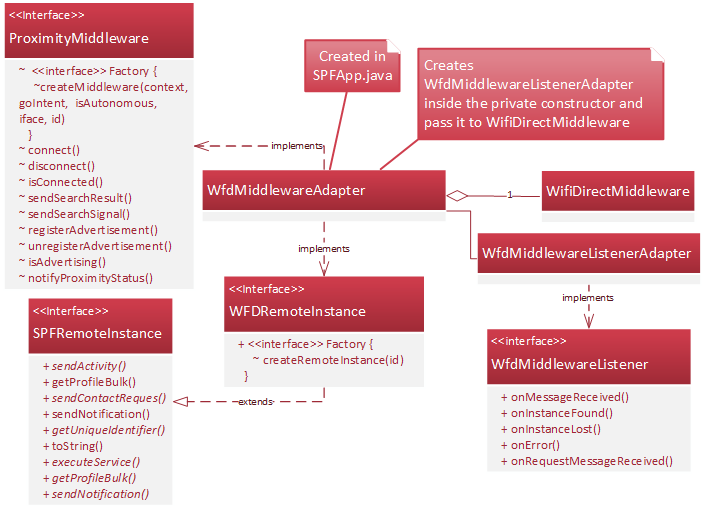
\includegraphics[scale=0.5]{./images/chap2/uml-parte1.png}
	\caption{Uml part 0.}
	\label{uml-part1}
\end{figure}	

\begin{figure}[thpb]
	\centering
	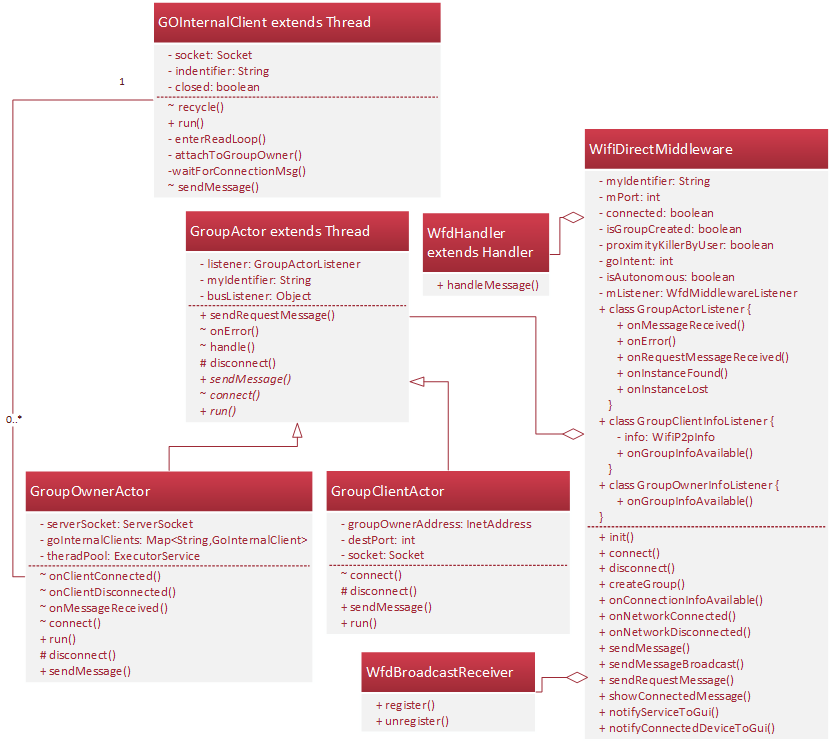
\includegraphics[scale=0.6]{./images/chap2/uml-parte2.png}
	\caption{Uml part 0.}
	\label{uml-part2}
\end{figure}	


Now, I want to explain quickly the class structure of this middleware. Because there is a huge number of classes, I selected only a subset of these, as you can see in Figures \ref{uml-part1} and \ref{uml-part2}.
I cannot and i don't want to explain in details all classes and methods, because it's impossibile. Also, i don't want to repeat the same things for GroupActor and its subclasses.
In this subsection, i want to explain some key feature of this new implementation of WifiDirectMiddleware.java.
In fact, there are some new important variable, like isAutonomous and goIntent. These variables are important, because chosen by the user from the UI. The first one is connected to the state of the switch ``Group Owner` and the second one to the switch ``Autonomous``. 
I implemented a quick workaround to achieve this, by passing variables during the creation of the Middleware and updating these values after every change to the switches states. Obviously, this is not good and I'll explain why into Section \ref{conclusion}.

%%%%add dome other informations describing these two figures

\section{Eternal Connect}

Eternal Connect is a solution to restart discovery and connect after some network errors. This can be considered an improved version of the Eternal Discovery that I used here https://github.com/deib-polimi/PigeonMessanger, because with this latest implementation, SPF will re-connect automatically trying every 15 second for 4 times. Obviously, you can configure this to achieve the best configurations. Also, you can improve Eternal Connect in different ways to obtain also better performances during network creation, in particular on the Group Owner in Autonomous mode.
All the code related to Eternal Connect is isolated into a single class called EternalConnect.java (instead of Pigeon Messenger, where the code was distributed in different classes).
Eternal Connect has two different modes:
\begin{enumerate}
	\item standard: with automatic reconnection in a loop cycle for 4 times every 15 seconds;
	\item simple: with a single automatic reconnection. If it fails, it will stop.
\end{enumerate}
These two modes are partially implemented, because I created only the necessary features. If you need a different behaviour you can simply modify \textsf{onEternalConnectUpdate} that catch EternalConnectEvent in WifiDirectMiddleware.java.

EternalConnect.java is a singleton class with these important public methods:
\begin{itemize}
	\item eternalConnect(): start the EternalConnect as you can see in Listing 	\ref{eternalConnect};
	\item onNetwork Disconnected(): if a device isn't a GO in Autonomous mode restarts the Eternal Connect, instead posts an EternalConnectEvent to specify the ``simple reconnection`` mode;
	\item onConnectFailed(): called when Wi-Fi Direct fails during the connection procedure, to restart the Eternal Connect in standard mode;
	\item onGroupCreationFailed(): called when Wi-Fi Direct fails during the group creation procedure, to restart the Eternal Connect in simple mode;
	\item eternalCompletedSuccessfully(): to complete the procedure, because the connection is established.
\end{itemize}


\begin{lstlisting}[caption={eternalConnect() method},label=eternalConnect, language=Java]
void eternalConnect(boolean proximityKilledByUser) {
	killScheduler();
    scheduler = Executors.newScheduledThreadPool(1);
    final Runnable runnable = new Runnable() {
    	public void run() {
        	if (proximityKilledByUser) {
        		killScheduler();
        		eternalCounter = 0;
            return;
        }	
		if (eternalCounter > MAX_ETERNAL_COUNT) {
        		killScheduler();
            eternalCounter = 0;
        } else {
        	  //post EternalConnectEvent.NEW_EC_CYCLE
            eternalCounter++;
        }
	}
};

final ScheduledFuture<?> eternalHandle =
	scheduler.scheduleAtFixedRate(runnable, 
		10, 15, TimeUnit.SECONDS);
    scheduler.schedule(new Runnable() {
    	public void run() {
          eternalHandle.cancel(true);
        }
    }, 15, TimeUnit.SECONDS);
}
\end{lstlisting}


\section{Wi-Fi Direct's known issues}

In this section i want to create a list will some of the known issues of Wi-Fi Direct protocol.
\begin{itemize}
	\item There are random errors (for example: 0 - bs) when you are trying to establish a connection. In most of the cases, to fix this problem you must kill the Wi-Fi Connection manually.
	\item The discovery procedure is absolutely unreliable. Sometime a device can't discover other devices without any reason and the only way to fix this problem is a stop followed by a restart of the discovery procedure.
	\item Connection between different devices with different Android versions and manufacturers can be unstable.
	\item The most important problem in SPF2 is related to autonomous group join operations. Because, if a device want to join to a previously created group should ask to the group owner of this group to join in. In Android API there isn't this concept (but in wpa\_supplicant yes, obviously), but there is the standard connect method. This is not a problem, instead the real problem is that in a device want to join shows a popup into the group owner. If the GO accept the join procedure can complete. This process can't be automated and always requires a user interaction. Also, for absolutely inexplicable reasons, when the connection with a third device starts, the entire group can be destroyed to try to recreate it quickly. This is a famous problem that you can found everywhere on stackoverflow and at the moment there aren't any solutions. If you want to use wpa\_supplicant from command line this problem never happens, this implies that is caused by the Android implementation of Wi-Fi Direct. Also, the main consequence related to this problem is that sometime the group won't be recreated, caused by fails during connection or discovery problem. To be able to create a group of three devices with SPF2 you should try some times to obtain the desired result. This is a huge pure Android's implementation issue.
\end{itemize}


